\begin{pa} \label{PA:11.1} 
  A group of ecologists would like to
  estimate the number of trees in a forest that is two miles long and
  one mile wide.  Rather than go through the forest counting every
  tree, they decide to visit sixteen locations and measure the
  {\em density} of trees---that is, the number of trees per
  square mile---in that location.

  Shown on the left in Figure \ref{F:11.1.forest} is the measured
  density in thousands of trees per square mile.  

  \begin{figure}[ht]
    \begin{center}
      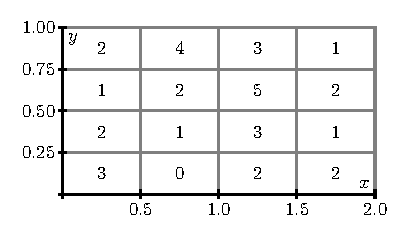
\includegraphics{figures/fig_11_1_forest.eps}
      \hspace*{20pt}
      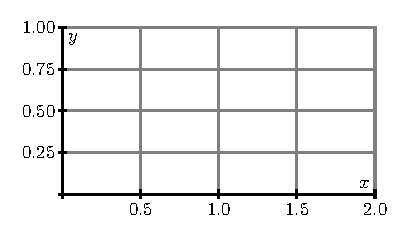
\includegraphics{figures/fig_11_1_forest_empty.eps}
    \end{center}
    \caption{The density of trees in the forest}
    \label{F:11.1.forest}
  \end{figure}

    \ba
    \item What is the area $\Delta A$ of each of the sixteen regions?
    \item If $f(x,y)$ measures the density of trees at location
      $(x,y)$, what is the meaning of $f(x,y)\Delta A$?
    \item Using the given densities, estimate the number of trees in
      each region and record your estimate on the right side of Figure
      \ref{F:11.1.forest}. 
    \item Estimate the number of trees in each of the four columns;
      that is, how many trees are there in each of the following
      ranges? 

      \medskip \noindent
      $\displaystyle 0 \leq x \leq 0.5$
      \hfill
      $\displaystyle 0.5 \leq x \leq 1.0$
      \hfill
      $\displaystyle 1.0 \leq x \leq 1.5$
      \hfill
      $\displaystyle 1.5 \leq x \leq 2.0$

      \item What is your estimate for the total number of trees in the
        forest? 

      \item How would you obtain a more accurate estimate?

      \item Instead of adding together the number of trees in each
        column, estimate the number of trees in each row:

        \medskip \noindent
        $\displaystyle 0 \leq y \leq 0.25$
        \hfill
        $\displaystyle 0.25 \leq y \leq0.5$
        \hfill
        $\displaystyle 0.5 \leq y \leq 0.75$
        \hfill
        $\displaystyle 0.75 \leq y \leq 1.0$

      \item Verify that you find the same estimate for the total
        number of trees in this way.


      \ea
\end{pa} \afterpa 